%% LyX 1.3 created this file.  For more info, see http://www.lyx.org/.
%% Do not edit unless you really know what you are doing.
\documentclass[english, 12pt]{article}
\usepackage{times}
%\usepackage{algorithm2e}
\usepackage{url}
\usepackage{bbm}
\usepackage[T1]{fontenc}
\usepackage[latin1]{inputenc}
\usepackage{geometry}
\geometry{verbose,letterpaper,tmargin=2.5cm,bmargin=2.5cm,lmargin=2.5cm,rmargin=2.5cm}
\usepackage{rotating}
\usepackage{color}
\usepackage{graphicx}
\usepackage{amsmath, amsthm, amssymb}
\usepackage{setspace}
\usepackage{lineno}
\usepackage{hyperref}
\usepackage{bbm}


\usepackage{xr}
\externaldocument{PRS-supp}

\linenumbers
\doublespacing
%\usepackage[authoryear]{natbib}
\usepackage{natbib} \bibpunct{(}{)}{;}{author-year}{}{,} 

%Pour les rajouts
\usepackage{color}
\definecolor{trustcolor}{rgb}{0,0,1}

\usepackage{dsfont}
\usepackage[warn]{textcomp}
\usepackage{adjustbox}
\usepackage{multirow}
\usepackage{graphicx}
\graphicspath{{../figures/}}
\DeclareMathOperator*{\argmin}{\arg\!\min}

\let\tabbeg\tabular
\let\tabend\endtabular
\renewenvironment{tabular}{\begin{adjustbox}{max width=\textwidth}\tabbeg}{\tabend\end{adjustbox}}

\makeatletter

%%%%%%%%%%%%%%%%%%%%%%%%%%%%%% LyX specific LaTeX commands.
%% Bold symbol macro for standard LaTeX users
%\newcommand{\boldsymbol}[1]{\mbox{\boldmath $#1$}}

%% Because html converters don't know tabularnewline
\providecommand{\tabularnewline}{\\}

\usepackage{babel}
\makeatother


\begin{document}


\title{Efficient implementation of penalized regression\\for genetic risk prediction}
\author{Florian Priv\'e,$^{\text{1,}*}$ Hugues Aschard$^{\text{2}}$ and Michael G.B. Blum$^{\text{1,}*}$}



\date{~ }
\maketitle

\noindent$^{\text{\sf 1}}$Laboratoire TIMC-IMAG, UMR 5525, Univ.\ Grenoble Alpes, CNRS, La Tronche (38700), France, \\
\noindent$^{\text{\sf 2}}$Centre de Bioinformatique, Biostatistique et Biologie Int\'egrative (C3BI), Institut Pasteur, Paris (75015), France.

\noindent$^\ast$To whom correspondence should be addressed.\\

\noindent Contacts: 
\begin{itemize}
\item \url{florian.prive@univ-grenoble-alpes.fr}
\item \url{hugues.aschard@pasteur.fr}
\item \url{michael.blum@univ-grenoble-alpes.fr}
\end{itemize}

\newpage

\abstract{
Polygenic Risk Scores (PRS) consist in combining the information across many single-nucleotide polymorphisms (SNPs) in a score reflecting the genetic risk of developing a disease. PRS might have a major impact on public health, possibly allowing for screening campaigns to identify high-genetic risk individuals for a given disease.  
The ``Clumping+Thresholding'' (C+T) approach is the most common method to derive PRS. C+T uses only univariate genome-wide association studies (GWAS) summary statistics, which makes it fast and easy to use. 
However, previous work showed that jointly estimating SNP effects for computing PRS has the potential to significantly improve the predictive performance of PRS as compared to C+T.

In this paper, we present an efficient method to jointly estimate SNP effects using individual-level data, allowing for practical application of penalized logistic regression (PLR) on modern datasets including hundreds of thousands of individuals. Moreover, our implementation of PLR directly includes automatic choices for hyper-parameters.

We compare the performance of PLR, C+T and a derivation of random forests using both real and simulated data. 
PLR consistently achieves higher predictive performance than the two other methods while being as fast as C+T. 
We find that improvement in predictive performance is more pronounced when there are few effects located in nearby genomic regions with correlated SNPs; for instance, AUC values increase from 83\% with the best prediction of C+T to 92.5\% with PLR. We confirm these results in a data analysis of a case-control study for celiac disease where PLR and the standard C+T method achieve AUC of 89\% and of 82.5\%.

In conclusion, our study demonstrates that penalized logistic regression can achieve more discriminative polygenic risk scores, while being applicable to large-scale individual-level data thanks to the implementation we provide in the R package bigstatsr.
}


%%%%%%%%%%%%%%%%%%%%%%%%%%%%%%%%%%%%%%%%%%%%%%%%%%%%%%%%%%%%%%%%%%%%%%%%%%%%%%%%

\newpage

\section{Introduction}

Polygenic Risk Scores (PRS) consist in combining the information across many single-nucleotide polymorphisms (SNPs) in a score reflecting the genetic risk of developing a disease. PRS are useful for genetic epidemiology when testing the polygenicity of one disease and finding a common genetic contribution between two diseases \cite[]{purcell2009common}. Personalized medicine is another major application of PRS. Personalized medicine envisions to use PRS in screening campaigns in order to identify high-risk individuals for a given disease \cite[]{chatterjee2016developing}. As an example of practical application, targeting screening to men at higher polygenic risk could reduce the problem of overdiagnosis and lead to a better benefit-to-harm balance in screening for prostate cancer \cite[]{pashayan2015implications}. 
Yet, PRS would have to show a high discriminative power between cases and controls in order to be used for helping in the diagnosis of diseases. For screening high-risk individuals and for presymptomatic diagnosis of the general population, it is suggested that the AUC must be greater than 75\% and 99\% respectively \cite[]{janssens2007impact}.

Several methods have been developed to predict disease status, or more generally any phenotype, based on SNP information. A commonly used method often called ``P+T'' or ``C+T'' (which stands for ``Clumping and Thresholding'') is used to derive PRS from results of Genome-Wide Association Studies (GWAS) \cite[]{chatterjee2013projecting,dudbridge2013power,evans2009harnessing,purcell2009common,wray2007prediction}. This technique uses GWAS summary statistics only, allowing for a fast implementation of C+T. However, C+T also has several limitations; for instance, previous studies have shown that predictive performance of C+T is very sensitive to the threshold of inclusion of SNPs, depending on the disease architecture \cite[]{ware2017heterogeneity}.
Linear Mixed-Models (LMMs) are another widely-used method in fields such as plant and animal breeding or for predicting highly heritable quantitative human phenotypes such as height \cite[]{yang2010common}. Yet, models resulting from LMM, known e.g.\ as ``gBLUP'', are not optimal for predicting disease status based on genotypes (see table 2 of \cite{abraham2013performance}), maybe because they were not primarily designed for this purpose. 
%Moreover, these methods and their derivatives are often computationally very demanding, both in terms of memory and time required, which makes them unlikely to be used for prediction on very large datasets \cite[]{golan2014effective,maier2015joint,speed2014multiblup,zhou2013polygenic}.
Finally, statistical learning methods have also been used to derive PRS for complex human diseases by jointly estimating SNP effects. Such methods include joint logistic regression, Support Vector Machine (SVM) and random forests \cite[]{abraham2012sparsnp,abraham2014accurate,botta2014exploiting,okser2014regularized,wei2009disease}.

We recently developed two R packages, bigstatsr and bigsnpr, for efficiently analyzing large-scale genome-wide data \cite[]{prive2017efficient}. Package bigstatsr now includes an efficient algorithm with a new implementation for computing sparse linear and logistic regressions on huge datasets as large as the UK Biobank \cite[]{bycroft2017genome}.
In this paper, we present a comprehensive comparative study of our implementation of penalized logistic regression (PLR) against the C+T method and the T-Trees algorithm, a derivation of random forests that has shown high predictive performance \cite[]{botta2014exploiting}.
In this comparison, we do not include any LMM method for the reasons mentioned before and do not include any SVM method because it is expected to give similar results to logistic regression \cite[]{abraham2012sparsnp}. 
For C+T, we report results for a large grid of hyper-parameters. 
For PLR, the choice of hyper-parameters is included in the algorithm so that we report only one model for each simulation. We also use a modified version of PLR in order to capture not only linear effects, but also recessive and dominant effects. 

To perform simulations, we use real genotype data and simulate new phenotypes. 
In order to make our comparison as comprehensive as possible, we compare different disease architectures by varying the number, size and location of causal effects as well as the disease heritability. We also compare two different models for simulating phenotypes, one with additive effects only, and one that combines additive, dominant and interaction-type effects.
Overall, we find that PLR achieves higher predictive performance than C+T except in highly underpowered cases (AUC values lower than 0.6), while being as fast. This demonstrates the feasibility and relevance of this approach for PRS computation based on large individual-level datasets that require scalable methods but offer some well power studies in return. 



%%%%%%%%%%%%%%%%%%%%%%%%%%%%%%%%%%%%%%%%%%%%%%%%%%%%%%%%%%%%%%%%%%%%%%%%%%%%%%%%

\section{Material and Methods}

\subsection{Genotype data}

We use real genotypes of European individuals from a case-control study for celiac disease \cite[]{dubois2010multiple}. The composition of this dataset is presented in table \ref{tab:celiac-data}. Details of quality control and imputation for this dataset are available in \cite{prive2017efficient}. For simulations presented later, we first restrict this dataset to controls from UK in order to remove the genetic structure induced by the celiac disease status and population structure. This filtering process results in a sample of 7100 individuals (see supplementary notebook ``preprocessing''). 
We also use this dataset for real data application, in this case keeping all 15,155 individuals (4496 cases and 10,659 controls). Both datasets contain 281,122 SNPs.

\subsection{Simulations of phenotypes} \label{sec:simus}

We simulate binary phenotypes using a Liability Threshold Model (LTM) with a prevalence of 30\% \cite[]{falconer1965inheritance}. We vary simulation parameters in order to match a range of genetic architectures from low to high polygenicity. 
This is achieved by varying the number of causal variants and their location (30, 300, or 3000 anywhere in all 22 autosomal chromosomes or 30 in the HLA region of chromosome 6), and the disease heritability $h^2$ (50\% or 80\%). 
%SNP effects are drawn from either a Gaussian or from a Laplace distribution.
Liability scores are computed either from a model with additive effects only (``ADD'') or a more complex model that combines additive, dominant and interaction-type effects (``COMP''). For model ``ADD'', we compute the liability score of the i-th individual \[y_i = \sum_{j\in S_\text{causal}} w_j \cdot \widetilde{G_{i,j}} ~~+~~ \epsilon_i~,\] where $S_\text{causal}$ is the set of causal SNPs, $w_j$ are weights generated from a Gaussian distribution $N(0, h^2 / \vert S_\text{causal} \vert)$ or a Laplace distribution $Laplace(0, \sqrt{h^2 / (2~\vert S_\text{causal} \vert)})$, $G_{i,j}$ is the allele count of individual $i$ for SNP $j$, $\widetilde{G_{i,j}}$ corresponds to its standardized version (zero mean and unit variance for all SNPs), and $\epsilon$ follows a Gaussian distribution $N(0, 1 - h^2)$.
For model ``COMP'', we simulate liability scores using additive, dominant and interaction-type effects (see Supplementary Materials).

We implement 3 different simulation scenarios, summarized in table \ref{tab:simus}.
Scenario \textnumero1 uses the whole dataset (all 22 autosomal chromosomes -- 281,122 SNPs) and a training set of size 6000. It compares all methods described in section \ref{sec:methods}. For each combination of the remaining parameters, results are based on 100 simulations except when comparing PLR with T-Trees, which relies on 5 simulations only because of a much higher computational burden of T-Trees as compared to other methods. 
Scenario \textnumero2 consists of 100 simulations per combination of parameters on a dataset composed of chromosome 6 only (18,941 SNPs). Reducing the number of SNPs increases the polygenicity (i.e.\ the proportion of causal SNPs) of the simulated models. Reducing the number of SNPs ($p$) is also equivalent to increasing the sample size ($n$) as predictive power is dependent on $n/p$ \cite[]{dudbridge2013power,vilhjalmsson2015modeling}. For this scenario, we use the additive model only, but continue to vary all other simulation parameters. 
Finally, scenario \textnumero3 uses the whole dataset as in scenario \textnumero1 while varying the size of the training set in order to assess how the sample size affects predictive performance of methods. A total of 100 simulations per combination of parameters are run using 300 causal SNPs randomly chosen on the genome.


\subsection{Predictive performance measures}\label{sec:auc}

In this study, we use two different measures of predictive accuracy. First, we use the Area Under the Receiver Operating Characteristic (ROC) Curve (AUC) \cite[]{fawcett2006introduction,lusted1971signal}. In the case of our study, the AUC is the probability that the PRS of a case is greater than the PRS of a control.
This measure indicates the extent to which we can distinguish between cases and controls using PRS. 
As a second measure, we also report the partial AUC for specificities between 90\% and 100\% \cite[]{dodd2003partial,mcclish1989analyzing}. This measure is similar to the AUC, but focuses on high specificities, which is the most useful part of the ROC curve in clinical settings. 
When reporting AUC results of simulations, we also report maximum achievable AUC values of 84\% and 94\% for heritabilities of 50\% and 80\% respectively. These estimates are based on three different yet consistent estimations (see Supplementary Materials). %Note that we also report the timing of the main computations and the number of SNPs used in the predictions.

\subsection{Methods compared} \label{sec:methods}

In this paper, we compare three different types of methods: the C+T method, T-Trees and penalized logistic regression (PLR).

The C+T (Clumping + Thresholding) method directly derives a Polygenic Risk Score (PRS) from the results of Genome-Wide Associations Studies (GWAS). In GWAS, a coefficient of regression (i.e.\ the estimated effect size $\hat\beta_j$) is learned independently for each SNP $j$ along with a corresponding p-value $p_j$. The SNPs are first clumped (C) so that there remain only loci that are weakly correlated with one another (this set of SNPs is denoted $S_\text{clumping}$). Then, thresholding (T) consists in removing SNPs with p-values larger than a user-defined threshold $p_T$. Finally, the PRS for individual $i$ is defined as the sum of allele counts of the remaining SNPs weighted by the corresponding effect coefficients \[\rm{PRS}_i = \sum_{\substack{j \in S_\text{clumping} \\ p_j~<~p_T}} \hat\beta_j \cdot G_{i,j}~,\] where $\hat\beta_j$ ($p_j$) are the effect sizes (p-values) learned from the GWAS. In this study, we mostly report scores for a clumping threshold at $r^2 > 0.2$ within regions of 500kb, but we also investigate thresholds of $0.05$ and $0.8$. We report three different scores of prediction: one including all the SNPs remaining after clumping (denoted ``C+T-all''), one including only the SNPs remaining after clumping and that have a p-value under the GWAS threshold of significance ($p < 5 \cdot 10^{-8}$, ``C+T-stringent''), and one that maximizes the AUC (``C+T-max'') for 102 p-value thresholds between $1$ and $10^{-100}$ (Table \ref{tab:thr}).
As we report the optimal threshold based on the test set, the AUC for ``C+T-max'' is an upper bound of the AUC for the C+T method.
For the computation of this paper, the GWAS part is done on the training set while clumping is done on the test set (all individuals not included in the training set).

T-Trees (\textit{Trees inside Trees}) is an algorithm derived from random forests \cite[]{breiman2001random} that takes into account the correlation structure among the genetic markers implied by linkage disequilibrium in GWAS data \cite[]{botta2014exploiting}. We use the same parameters as reported in Table 4 of \cite{botta2014exploiting}, except that we use 100 trees instead of 1000. Using 1000 trees provides a minimal increase of AUC while requiring a disproportionately long processing time (e.g.\ AUC of 81.5\% instead of 81\%, data not shown). %We call this method ``T-Trees'' in the results.

Finally, for penalized logistic regression (PLR), we find regression coefficients $\beta_0$ and $\beta$ that minimize the following regularized loss function \[L(\lambda, \alpha) = \underbrace{ -\sum_{i=1}^n \left( y_i \log\left(z_i\right) + (1 - y_i) \log\left(1 - z_i\right) \right) }_\text{Loss function}   +   \underbrace{ \lambda \left((1-\alpha)\frac{1}{2}\|\beta\|_2^2 + \alpha \|\beta\|_1\right) }_\text{Penalization} ~,\] where $z_i=1/\left(1+\exp\left(-(\beta_0 + x_i^T\beta)\right)\right)$, $x$ is denoting the genotypes and covariables (e.g.\ principal components), $y$ is the disease status to predict, $\lambda$ and $\alpha$ are two regularization hyper-parameters that need to be chosen.
Different regularizations can be used to prevent overfitting, among other benefits: the L2-regularization (``ridge'', \cite{hoerl1970ridge}) shrinks coefficients and is ideal if there are many predictors drawn from a Gaussian distribution (corresponds to $\alpha = 0$ in the previous equation);
the L1-regularization (``lasso'', \cite{tibshirani1996regression}) forces some of the coefficients to be equal to zero and can be used as a means of variable selection, leading to sparse models (corresponds to $\alpha = 1$);
the L1- and L2-regularization (``elastic-net'', \cite{zou2005regularization}) is a compromise between the two previous penalties and is particularly useful in the $p \gg n$ situation ($p$ is the number of SNPs), or any situation involving many correlated predictors (corresponds to $0 < \alpha < 1$) \cite[]{friedman2010regularization}. In this study, we use an embedded grid search over $\alpha \in \{1,~0.5,~0.05,~0.001\}$.

To fit this penalized logistic regression, we use an efficient algorithm \cite[]{friedman2010regularization,tibshirani2012strong,zeng2017efficient} from which we derived our own implementation in R package bigstatsr.
This type of algorithm builds predictions for many values of $\lambda$, which is called a ``regularization path''. To obtain an algorithm free of the choice of this hyper-parameter $\lambda$, we developed a procedure that we call Cross-Model Selection and Averaging (CMSA, figure \ref{fig:CMSA}).
Because of L1-regularization, the resulting vectors of coefficients are sparse and can be used to make a PRS based on a \emph{linear} combination of allele counts. We refer to this method as ``PLR'' in the results section.

To capture recessive and dominant effects on top of additive effects in PLR, we use simple feature engineering: we construct a separate dataset with 3 times as many variables as the initial one. 
For each SNP variable, we add two more variables coding for recessive and dominant effects: one variable is coded 1 if homozygous variant and 0 otherwise, and the other is coded 0 for homozygous referent and 1 otherwise.
We then apply our PLR implementation to this dataset with 3 times as many variables as the initial one; we refer to this method as ``PLR3'' in the rest of the paper.

\subsection{Evaluating predictive performance for Celiac data}

We use Monte Carlo cross-validation to compute AUC, partial AUC, the number of predictors and execution time for the original Celiac dataset with the observed case-control status: we randomly split 100 times the dataset in a training set of 12,000 individuals and a test set composed of the remaining 3155 individuals.

%%%%%%%%%%%%%%%%%%%%%%%%%%%%%%%%%%%%%%%%%%%%%%%%%%%%%%%%%%%%%%%%%%%%%%%%%%%%%%%%

\section{Results}

\subsection{Joint estimation improves predictive performance}

We compared penalized logistic regression (PLR) with the C+T method using simulations of scenario \textnumero1 (Table \ref{tab:simus}).
When simulating a model with 30 causal SNPs and an heritability of 80\%, PLR provides AUC of 93\%, nearly reaching the maximum achievable AUC of 94\% for this setting (Figure \ref{fig:main-AUC-logit}). 
Moreover, PLR consistently provides higher predictive performance than C+T across all scenarios we considered, except in some cases of high polygenicity or small sample size where all methods perform poorly (AUC values below 60\% -- figures \ref{fig:main-AUC-ntrain} and \ref{fig:supp-AUC-logit}).
PLR provides particularly higher predictive performance than C+T when there are correlations between predictors, i.e.\ when we choose causal SNPs to be in the HLA region. In this situation, the mean AUC reaches 92.5\% for PLR and 84\% for ``C+T-max'' (Figure \ref{fig:main-AUC-logit}).
Note that, for the simulations, we do not report results in terms of partial AUC because partial AUC values have a Spearman correlation of 98\% with the AUC results for all methods (Figure \ref{fig:supp-AUC-corr}).

\subsection{Importance of hyper-parameters}

In practice, a particular value of the threshold of inclusion of SNPs should be chosen for the C+T method and this choice can dramatically impact the predictive performance of C+T. 
For example, in a model with 30 causal SNPs, AUC ranges from less than 60\% when using all SNPs passing clumping to 90\% \emph{if} choosing the optimal p-value threshold (Figures \ref{fig:main-AUC-PRS} and \ref{fig:supp-AUC-PRS}).

Concerning the $r^2$ threshold of the clumping step in C+T, we mostly used the common value of $0.2$. Yet, using a more stringent value of $0.05$ provides higher predictive performance than using $0.2$ in most of the cases we considered (Figures \ref{fig:supp-AUC-all-r2}, \ref{fig:main-AUC-ntrain} and \ref{fig:supp-AUC-chr6-all-r2})

Our implementation of PLR that automatically chooses hyper-parameter $\lambda$ provides similar predictive performance than the best predictive performance of 100 models corresponding to different values of $\lambda$ (Figure \ref{fig:supp-biglasso}).


\subsection{Non-linear effects}

We tested the T-Trees method in scenario \textnumero1.
As compared to PLR, T-Trees perform worse in terms of predictive ability, while taking much longer to run (Figure \ref{fig:supp-ttrees}). 
Even for simulations with model ``COMP'' in which there are dominant and interaction-type effects that T-Trees should be able to handle, AUC is still lower when using T-Trees than when using PLR (Figure \ref{fig:supp-ttrees}).

We also compared the two penalized logistic regressions in scenario \textnumero1: PLR versus PLR3 that uses additional features (variables) coding for recessive and dominant effects.
Predictive performance of PLR3 are nearly as good as PLR when there are additive effects only (differences of AUC are always smaller than 2\%) and can lead to significantly greater results when there are also dominant and interactions effects (Figures \ref{fig:supp-triple} and \ref{fig:supp-AUC-triple}). For model ``COMP'', PLR3 provides AUC values at least 3.5\% higher than PLR, except when there are 3000 causal SNPs.
Yet, PLR3 takes 2-3 times as much time to run and requires 3 times as much disk storage as PLR.

\subsection{Simulations varying number of SNPs and training size} %%%%

First, when reproducing simulations of scenario \textnumero1 using chromosome 6 only (scenario \textnumero2), the predictive performance of PLR always increase (Figure \ref{fig:supp-AUC-chr6-all-r2}). 
There is a particularly large increase when simulating 3000 causal SNPs: AUC from PLR increases from 60\% to nearly 80\% for Gaussian effects and a disease heritability of 80\%.
On the contrary, when simulating only 30 or 300 causal SNPs with the corresponding dataset, AUC of ``C+T-max'' does not increase, and even decreases for an heritability of 80\% (Figure \ref{fig:supp-AUC-chr6-all-r2}). 
Secondly, when varying the training size (scenario \textnumero3), we report an increase of AUC with a larger training size, with a faster increase of AUC for PLR as compared to ``C+T-max'' (Figure  \ref{fig:main-AUC-ntrain}).


\subsection{Polygenic scores for the celiac disease}

Joint logistic regressions also provide higher AUC values for the Celiac data: 88.7\% with PLR and 89.1\% with PLR3 as compared to 82.5\% with ``C+T-max''.
The relative increase in partial AUC, for specificities larger than 90\%, is even larger (42\% and 47\%) with partial AUC values of 0.0411, 0.0426 and 0.0289 obtained with PLR, PLR3 and ``C+T-max'', respectively.
Moreover, logistic regressions use less predictors, respectively 1570, 2260 and 8360 (Table \ref{tab:results-celiac}, figure \ref{fig:celiac-roc} and supplementary notebook ``results-celiac'').
In terms of computation time, we show that PLR, while learning jointly on all SNPs at once and testing four different values for hyper-parameter $\alpha$, is almost as fast as the C+T method (190 vs 130 seconds), and PLR3 takes less than twice as long as PLR (296 vs 190 seconds). Finally, on this Celiac dataset, our implementation of PLR runs 300 times as fast as SparSNP \cite[]{abraham2012sparsnp}.

\begin{table}[h]
\caption{Results for the real Celiac dataset. The results are averaged over 100 runs where the training step is randomly composed of 12,000 individuals. In the parentheses is reported the standard deviation of $10^5$ bootstrap samples of the mean of the corresponding variable. Results are reported with 3 significant digits.\label{tab:results-celiac}}
\vspace*{0.5em}
\centering
\begin{tabular}{|l|c|c|c|c|}
  \hline
Method & AUC & pAUC & \# predictors & Execution time (s) \\
  \hline
C+T-max & 0.825 (0.000664) & 0.0289 (0.000187) & 8360 (744) & 130 (0.143) \\ 
PLR & 0.887 (0.00061) & 0.0411 (0.000224) & 1570 (46.4) & 190 (1.21) \\ 
PLR3 & 0.891 (0.000628) & 0.0426 (0.000219) & 2260 (56.1) & 296 (2.03) \\ 
   \hline
\end{tabular}
\end{table}

\subsection{Penalized regression for the UK Biobank}

We tested our implementation on 656K genotyped SNPs of the UK Biobank, keeping only caucasian individuals and removing individuals related to someone else in the data (second individual in each pair with a kinship greater than 0.08). Our L1-penalized linear regression runs in less than one day for 350K individuals, achieving a correlation of 65.5\% with true height for both sexes. The best C+T model achieves a correlation of 55\% for women and 56\% for men, where the GWAS part takes 1 hour only.
Our L1-penalized logistic regression on breast cancer runs in only 12 minutes for 150K women, achieving an AUC of 0.587. The best C+T model achieves the same AUC score, where the GWAS part takes 15 hours.



%%%%%%%%%%%%%%%%%%%%%%%%%%%%%%%%%%%%%%%%%%%%%%%%%%%%%%%%%%%%%%%%%%%%%%%%%%%%%%%%

\section{Discussion}

\subsection{Time and memory requirements}

The computation time of our PLR implementation mainly depends on the sample size and the number of active variables. Indeed, the algorithm is composed of two steps: first, for each variable, the algorithm computes one statistic that will be used to decide if the variable enters the model or not. Then, the algorithm iterates over a regularization path of decreasing values of $\lambda$, which progressively enables variables to enter the model (Figure  \ref{fig:CMSA}). So, in the second step, the number of variables is increasing progressively, and at some point the computation stops due to the early stopping criterion (prediction is getting worse on the corresponding validation set, see figure \ref{fig:CMSA}).

So, for highly polygenic traits such as height and when using huge datasets such as the UK Biobank, the algorithm might iterate over dozens of thousands of variables, which takes time (but still less than one day with our implementation). On the contrary, for traits like the celiac disease or breast cancer that seems to be less polygenic, a lot less variables are entering the model and the fitting is very fast (12 minutes only for 150K women of the UK Biobank for breast cancer!). Using more cases (there were only 3542 for Celiac and 6374 for Breast Cancer), one might achieve better predictive performance for these two diseases, and the computation time should stay within a few hours.

Regarding memory requirements, this is basically the same as for computation time. Indeed, active variables are accessed in memory thanks to memory-mapping when they are used \cite[]{prive2017efficient}. If there are too many variables accessed, the operating system (OS) has to make some space for new comping variables. So, there should never be any memory issue thanks to memory-mapping, yet, at some point, if there are too many active variables, the OS would regularly swap memory between disk and RAM, which is very slow. If this happens for very large datasets, you can try to use less processing cores (as active sets tend to have non-overlapping variables because of LD) or buy more RAM. We have quickly tested processing each chromosome separately and then combining the models later but this did not seem to perform as well as fitting all SNPs at once.

\subsection{Joint estimation improves predictive performance}

In this comparative study, we present a computationally efficient implementation of penalized logistic regression (PLR). 
This model can be used to build polygenic risk scores based on very large individual-level SNP datasets such as the UK biobank \cite[]{bycroft2017genome}. 
In agreement with previous work \cite[]{abraham2013performance}, we show that jointly estimating SNP effects has the potential to substantially improve predictive performance as compared to the standard C+T approach in which SNP effects are learned independently. 
PLR always outperforms the C+T method, except in some highly underpowered cases (AUC values always less than 0.6), and the benefits of using PLR are more pronounced with an increasing sample size or when causal SNPs are correlated with one another (Figures \ref{fig:supp-AUC-chr6-all-r2} and \ref{fig:main-AUC-ntrain}). 
This could be explained by the fact that PLR is too conservative in underpowered cases.

\subsection{Importance of hyper-parameters}

The choice of hyper-parameter values is very important since it can greatly impact method performance. In the C+T method, there are two main hyper-parameters: the $r^2$ and the $p_T$ thresholds that control how stringent are the clumping and thresholding steps, respectively. 
The choice of the $r^2$ threshold of the clumping step is important. 
Indeed, on the one hand, choosing a low value for this threshold may discard informative SNPs that are correlated.
Yet, on the other hand, when choosing a high value for this threshold, too much redundant information would be included in the model, which would add some noise to the PRS.
Based on the simulations, we find that using a stringent threshold ($r^2 = 0.05$) leads to higher predictive performance, even when causal SNPs are correlated. It means that, in most cases tested in this paper, avoiding redundant information is more important than including all causal SNPs.
The choice of the $p_T$ threshold is also very important as it can greatly impact the predictive performance of the C+T method, which we confirm in this study \cite[]{ware2017heterogeneity}. 
In this paper, we reported the maximum AUC of 102 different p-value thresholds, a threshold that should normally be learned on the training set only. To our knowledge, there is no clear standard on how to choose these two critical hyper-parameters for C+T. 
We did not want to choose the C+T parameters so that one could not criticize the procedure we would have used. Instead, for C+T, we chose to report the best AUC value on the test set, even if it leads to over-optimistic results for C+T as compared to PLR.


In contrast, for the penalized logistic regression presented here, we developed an automatic procedure called Cross-Model Selection and Averaging (CMSA) that releases investigators from the burden of choosing hyper-parameter $\lambda$ that accounts for the amount of regularization used in the model. Not only this procedure provides near-optimal results, but it also accelerates the model training thanks to the development of an early stopping criterion. 
Usually, cross-validation is used to choose hyper-parameter values and then the model is trained again with these particular hyper-parameter values \cite[]{Hastie2008,wei2013large}. Yet, performing cross-validation and retraining the model is computationally demanding; CMSA offers a less burdensome alternative. 
Concerning hyper-parameter $\alpha$ that accounts for the relative importance of the L1 and L2 regularizations, we use a grid  search directly embedded in the CMSA procedure. 
%Our penalized logistic regression implementation does not allow for setting $\alpha = 0$, a model that would assume the infinitesimal model. Yet, if using e.g.\ $\alpha = 0.001$, it would lead to a similar model.

\subsection{Non-linear effects}

We also explored how to capture non-linear effects. For this, we introduced a simple feature engineering technique that enables PLR to detect and learn not only additive effects, but also dominant and recessive effects. 
This technique improves the predictive performance of PLR when there are some non-linear effects in the simulations, while providing nearly the same predictive performance when there are additive effects only. 
Moreover, it also improves predictive performance for the celiac disease. 

Yet, this approach is not able to detect interaction-type effects. 
In order to capture interaction-type effects, we tested T-Trees, a method that is able to exploit SNP correlations and interactions thanks to special decision trees \cite[]{botta2014exploiting}. 
However, predictive performance of T-Trees are consistently lower than with penalized logistic regression, even when simulating a model with dominant and interaction-type effects that T-Trees should be able to handle.

\subsection{Limitations}

Our approach has one major limitation: the main advantage of the C+T method is its direct applicability to summary statistics, allowing to leverage the largest GWAS results to date, even when individual cohort data cannot be merged because of practical or ethical reasons (e.g.\ consortium data including many cohorts). As of today, our penalized logistic regression does not allow for the analysis of summary data, but this represents an important future direction of our work. 
The current version is of particular interest for the analysis of modern individual-level datasets including hundreds of thousands of individuals. 

Finally, in this comparative study, we did not consider the problem of population structure \cite[]{marquez2017multiethnic,martin2017human,vilhjalmsson2015modeling} and also did not consider non-genetic data such as environmental and clinical data \cite[]{dey2013integration,van2012integration}. 
%In future work, we aim at exploring how we can overcome those issues.
%We will use a dataset as large as the UK biobank \cite[]{bycroft2017genome}. Finally, we also wish to assess how can we combine the information provided by genetic data with clinical and environmental data, possibly in a non-linear way.

\subsection{Conclusion}

In this comparative study, we have presented a computationally efficient implementation of penalized logistic regression that can be used to predict disease status based on genotypes. Note that a similar penalized linear regression is also available in our software. Our approach solves the dramatic computational burden faced by standard implementations, thus allowing for the analysis of large-scale datasets such as the UK biobank \cite[]{bycroft2017genome}. 

We also demonstrated in simulations and real datasets that our implementation of penalized regressions is highly effective over a broad range of disease architectures. It can be appropriate for predicting autoimmune diseases with a few strong effects (e.g.\ celiac disease) as well as highly polygenic traits (e.g.\ standing height).  Finally, note that these models could also be used to predict phenotypes based on other omics data since the implementation is not specific to genotype data.


%%%%%%%%%%%%%%%%%%%%%%%%%%%%%%%%%%%%%%%%%%%%%%%%%%%%%%%%%%%%%%%%%%%%%%%%%%%%%%%%
%%%%%%%%%%%%%%%%%%%%%%%%%%%%%%%%%%%%%%%%%%%%%%%%%%%%%%%%%%%%%%%%%%%%%%%%%%%%%%%%

\newpage
\begin{table}[htbp]
\caption{Summary of all simulations. Where there is symbol `-' in a box, it means that the parameters are the same as the ones in the upper box.\label{tab:simus}}
\vspace*{0.5em}
\centering
\begin{tabular}{|c|c|c|c|c|c|c|c|}
\hline
Numero of & \multirow{2}{*}{Dataset} & Size of & Causal SNPs & Distribution & \multirow{2}{*}{Heritability} & Simulation & \multirow{2}{*}{Methods} \\ 
scenario & & training set & (number and location) & of effects & & model & \\
\hline
\hline
\multirow{4}{*}{1} & \multirow{4}{*}{All 22 chromosomes} & \multirow{4}{*}{6000} & 30 in HLA & \multirow{2.5}{*}{Gaussian} & \multirow{2.5}{*}{0.5} & \multirow{2.5}{*}{ADD} & C+T \\
& & & 30 in all & & & & PLR \\
& & & 300 in all & \multirow{1.5}{*}{Laplace} & \multirow{1.5}{*}{0.8} & \multirow{1.5}{*}{COMP} & PLR3 \\
& & & 3000 in all & & & & (T-Trees) \\
\hline
\multirow{2}{*}{2} & \multirow{2}{*}{Chromosome 6 only} & \multirow{2}{*}{-} & \multirow{2}{*}{-} & \multirow{2}{*}{-} & \multirow{2}{*}{-} & \multirow{2}{*}{ADD} & C+T \\ 
& & & & & & & PLR\\
\hline
\multirow{5}{*}{3} & \multirow{5}{*}{All 22 chromosomes} & 1000 & \multirow{5}{*}{300 in all} & \multirow{5}{*}{-} & \multirow{5}{*}{-} & \multirow{5}{*}{-} & \multirow{5}{*}{-} \\ 
& & 2000 & & & & & \\
& & 3000 & & & & & \\
& & 4000 & & & & & \\
& & 5000 & & & & & \\
\hline
\end{tabular}
\end{table}


\newpage
\begin{figure}[h]
\centerline{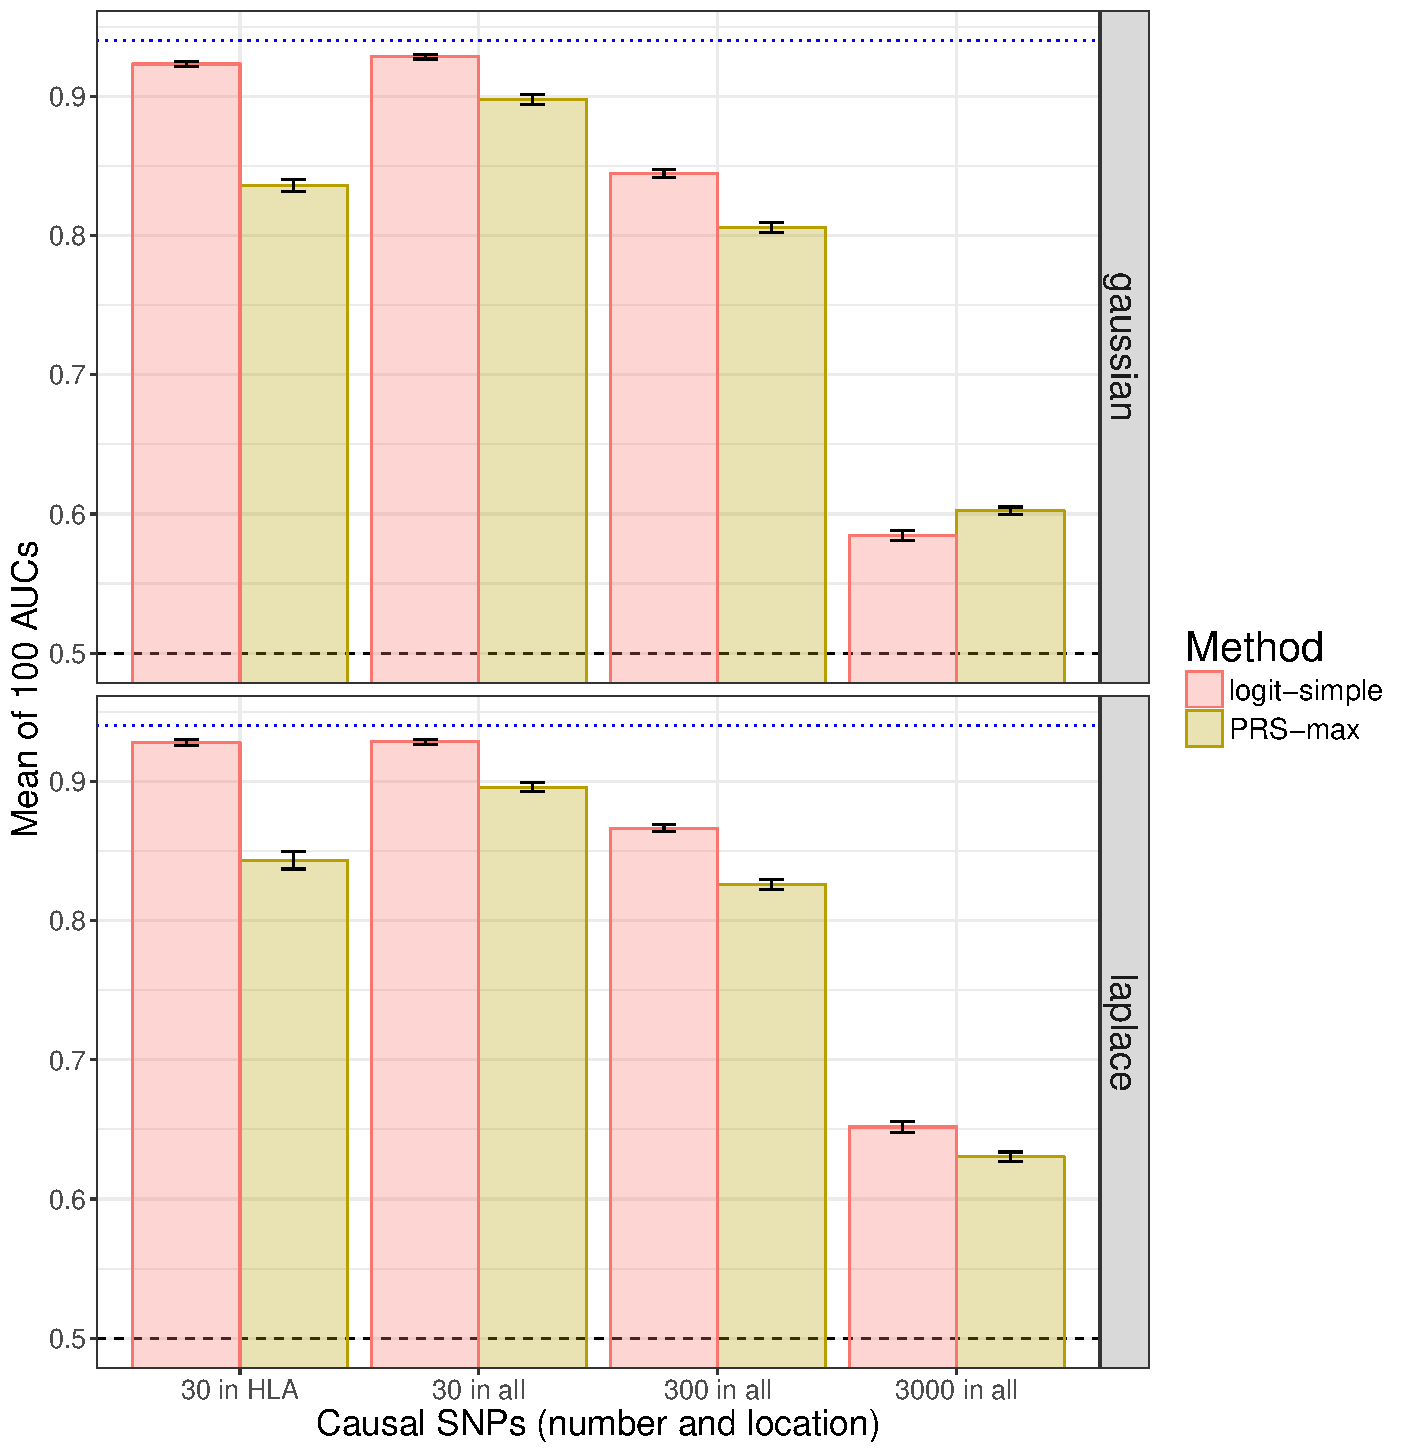
\includegraphics[width=\textwidth]{main-AUC-logit}}
\caption{Main comparison of C+T and PLR in scenario \textnumero1 for model ``ADD'' and an heritability of 80\%. Mean AUC over 100 simulations for PLR and the maximum AUC reported with ``C+T-max''. Upper (lower) panel is presenting results for effects following a Gaussian (Laplace) distribution. Error bars are representing $\pm 2 \text{SD}$ of $10^5$ non-parametric bootstrap of the mean AUC. The blue dotted line represents the maximum achievable AUC.}
\label{fig:main-AUC-logit}
\end{figure}

\newpage
\begin{figure}[h]
\centerline{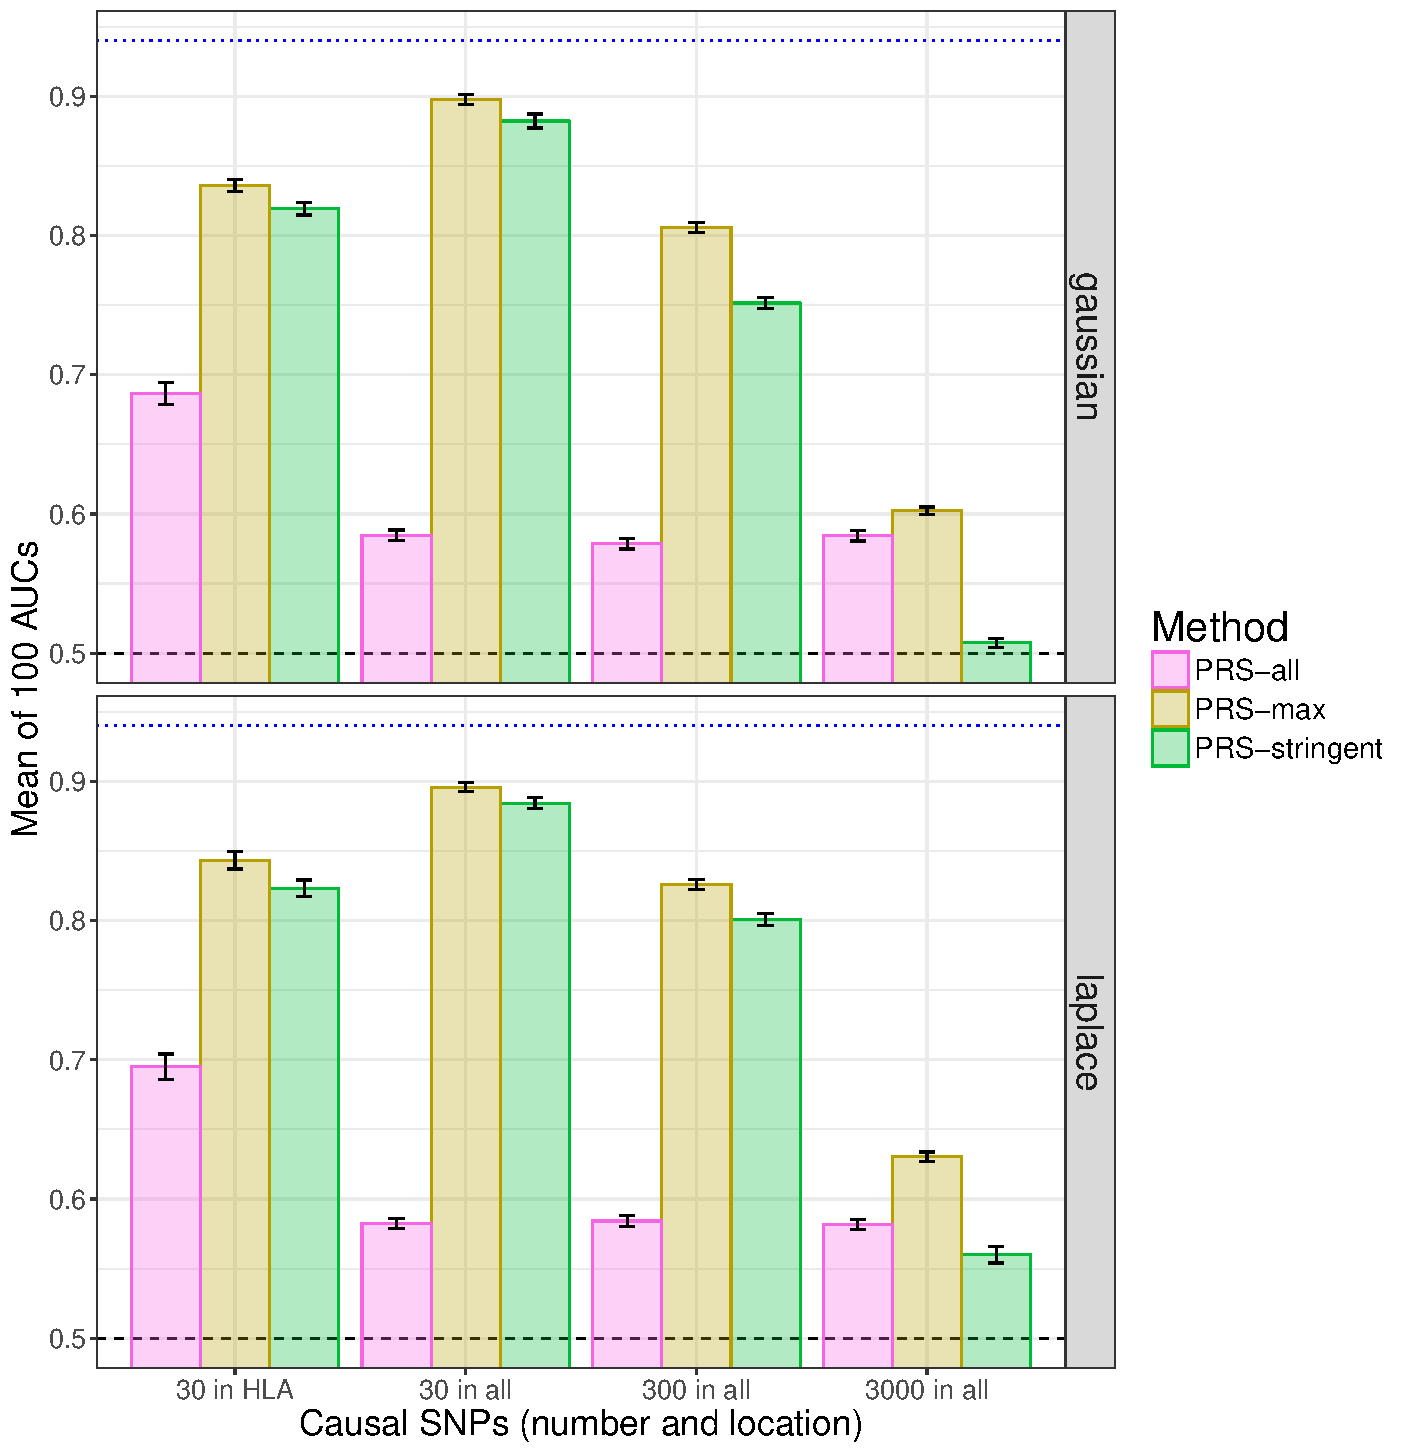
\includegraphics[width=\textwidth]{main-AUC-PRS}}
\caption{Comparison of three different p-value thresholds used in the C+T method in scenario \textnumero1 for model ``ADD'' and an heritability of 80\%. Mean AUC over 100 simulations. Upper (lower) panel is presenting results for effects following a Gaussian (Laplace) distribution. Error bars are representing $\pm 2 \text{SD}$ of $10^5$ non-parametric bootstrap of the mean AUC. The blue dotted line represents the maximum achievable AUC.}
\label{fig:main-AUC-PRS}
\end{figure}

\newpage
\begin{figure}[h]
\centerline{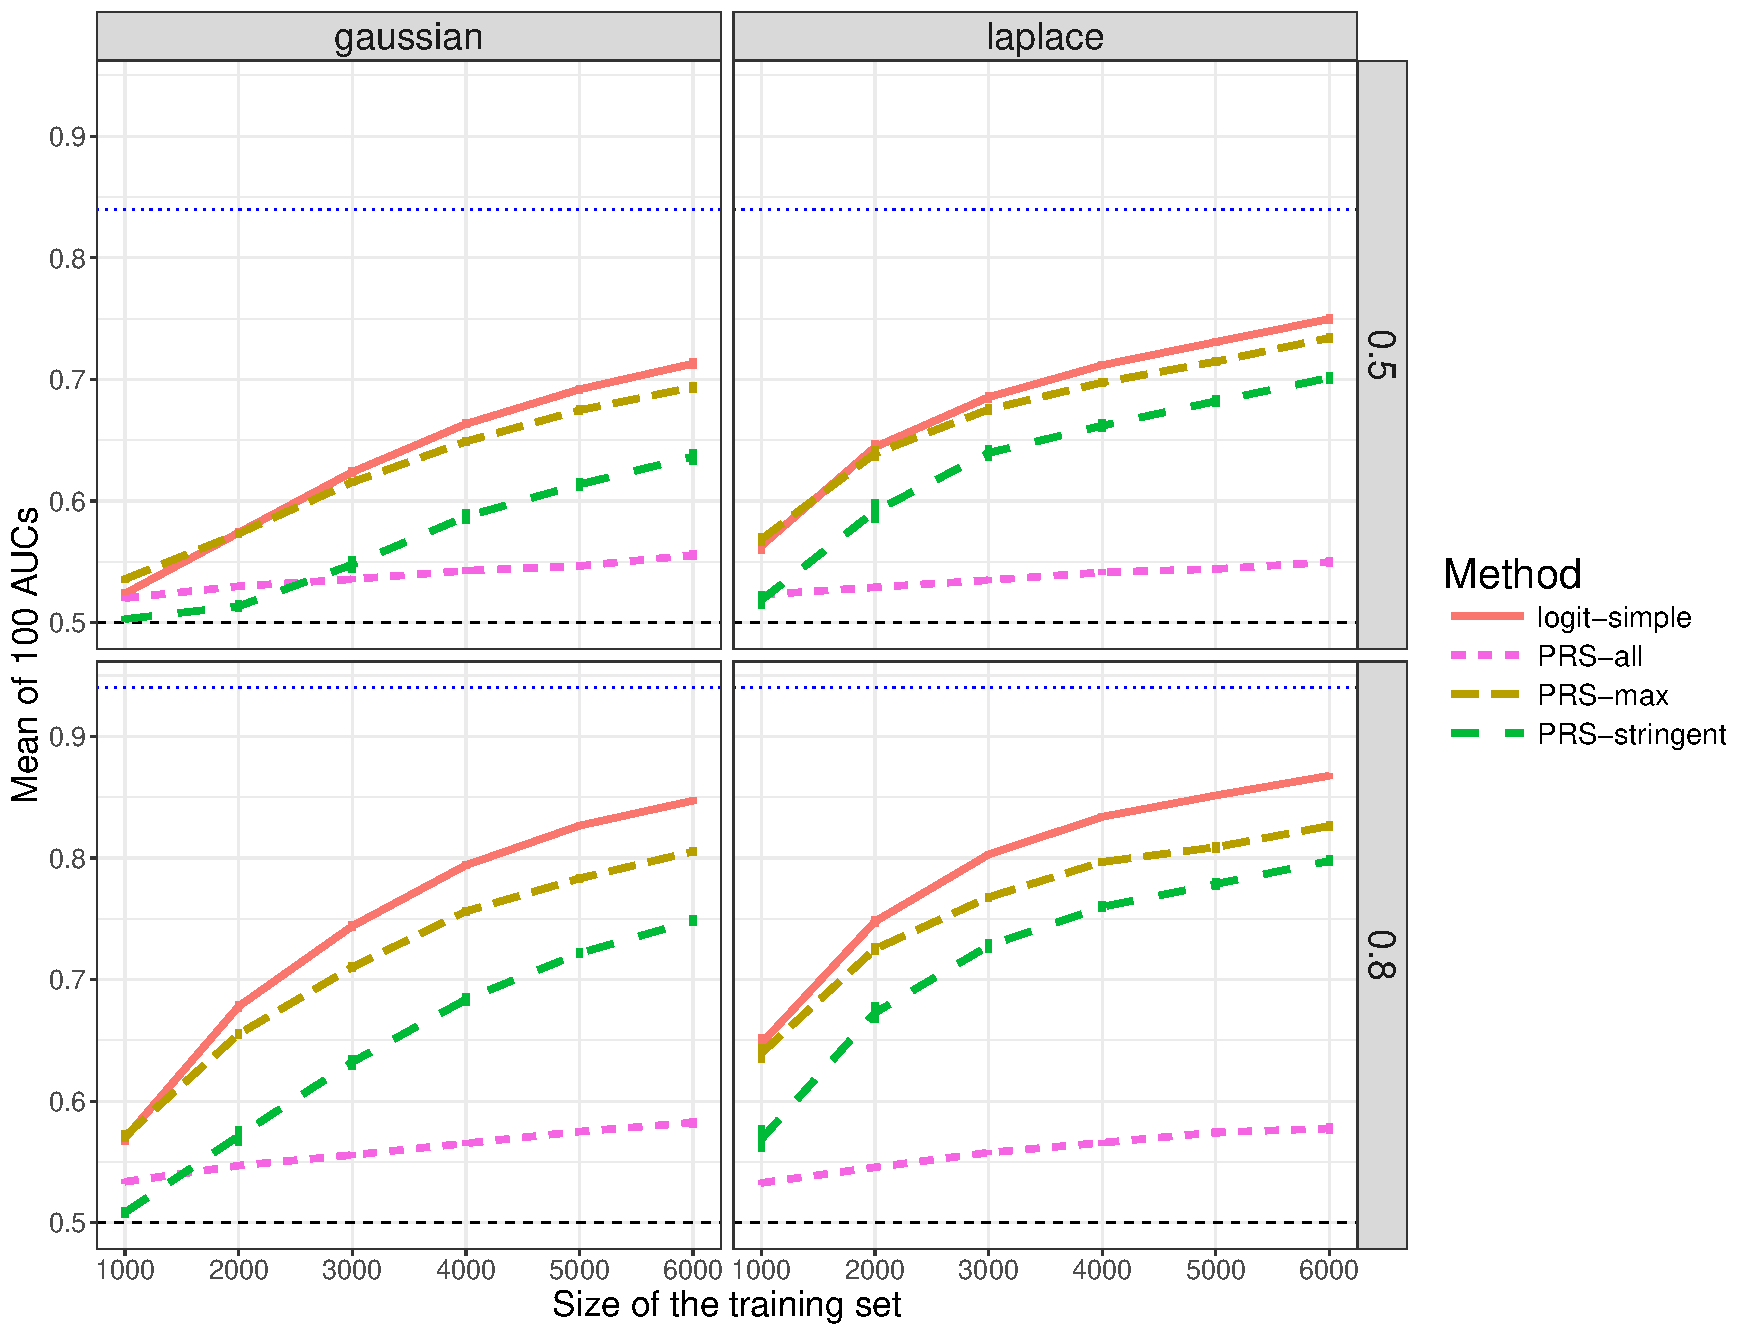
\includegraphics[width=\textwidth]{main-AUC-ntrain}}
\caption{Comparison of methods when varying sample size in scenario \textnumero3 for model ``ADD'' with 300 causal SNPs sampled anywhere on the genome. Mean AUC over 100 simulations for the maximum values of C+T for three different $r^2$ thresholds ($0.05$, $0.2$ and $0.8$) and PLR as a function of the training size. Upper (lower) panels are presenting results for effects following a Gaussian (Laplace) distribution and left (right) panels are presenting results for an heritability of 0.5 (0.8). Error bars are representing $\pm 2 \text{SD}$ of $10^5$ non-parametric bootstrap of the mean AUC. The blue dotted line represents the maximum achievable AUC.}
\label{fig:main-AUC-ntrain}
\end{figure}

\newpage
\begin{figure}[h]
\centerline{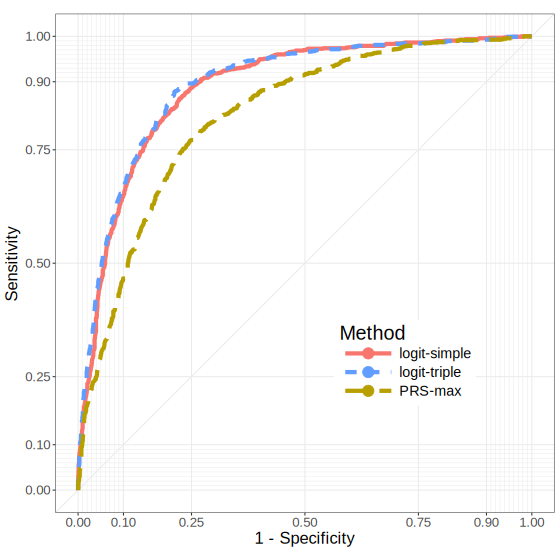
\includegraphics[width=\textwidth]{celiac-roc}}
\caption{ROC Curves for C+T, PLR and PLR3 for the celiac disease dataset. Models were trained using 12,000 individuals. These are results projecting these models on the remaining 3155 individuals. The figure is plotted using R package plotROC \cite[]{sachs2017plotroc}.\label{fig:celiac-roc}}
\end{figure}

%%%%%%%%%%%%%%%%%%%%%%%%%%%%%%%%%%%%%%%%%%%%%%%%%%%%%%%%%%%%%%%%%%%%%%%%%%%%%%%%

\clearpage

\section*{Description of Supplemental Data}

Supplemental Data include a PDF with two sections of methods, two tables and ten figures. 
Supplemental Data also include six HTML R notebooks including all code and results used in this paper, for reproducibility purposes, and available at \url{https://figshare.com/articles/code/7178750}.

\section*{Declaration of Interests}

The authors declare no competing interests.

\section*{Acknowledgements}

Authors acknowledge LabEx PERSYVAL-Lab (ANR-11-LABX-0025-01). Authors also acknowledge the Grenoble Alpes Data Institute that is supported by the French National Research Agency under the ``Investissements d'avenir'' program (ANR-15-IDEX-02).
We used the UK Biobank resource (application ID 25589).
We are also grateful to F\'elix Balazard for useful discussions about T-Trees, and to Yaohui Zeng for useful discussions about R package biglasso.
Finally, we are grateful to the two anonymous reviewers who contributed to improving this paper.

\section*{Web Resources}

Results of simulations are available at \url{https://figshare.com/articles/results_zip/7126964}. A tutorial on how to start with R packages bigstatsr and bigsnpr is available at \url{https://privefl.github.io/bigsnpr/articles/demo.html}. The two R packages are available on GitHub.

\newpage

\bibliographystyle{natbib}
\bibliography{refs}

\end{document}
